\chapter{Princip fungování regulárních výrazů}\label{sec:Principle}

Abychom mohli porozumět, jakým problémem se v této práci budeme zabývat, musíme si zadefinovat co jsou
regulární výrazy, jak fungují a jak se jednotlivé implementace mohu lišit. Následovně si vysvětlíme, jak lze zjednodušit
pochopení těchto výrazů, popřípadě jak rychle najít chybu ve vlastním výrazu. 

\section{Definice}
Předtím než si vysvětlíme blíže jak fungují samotné regulární výrazy, je potřeba si první objasnit význam několika pojmů z teoretické informatiky.
Regulární jazyky jsou jednou z možných definic formálních jazyků.

Formální jazyk je libovolná množina koečných slov nad určitou abecedou. Slova chápeme jako retězece znaků, která jsou příjimaná zadaným jazykem.
Tato slova musí být sice konečná ale množina těchto slov může být nekonečná. Tyto jazyky mohou být definovány regulárními výrazy, formální gramatikou, konečnými automaty a dalšími.

Ve spojení regulárních výrazu se často vyskytují konečné automaty, jedná se o další oblast v teoretické informatice.
Proto abychom pochopili proč je tato oblast pro nás důležitá, musíme si vysvětlit co vlastně jsou.

Konečné automaty popisují jsou modely jednoduchého počítače, který má určitý počet stavů a přechodů \cite{Havrlant}. 
Dělíme je na deterministické a nedeterministické, zkráceně DFA (deterministic finite automata) a NDA (non-deterministic finite automata).
Deterministické automaty mohou mít v daném stavů pro každý znak abecedy maximálně jeden přechod, dále nemohou obsahovat tzv. prázný znak často označovaný řeckým písmenem epsilon $\epsilon$.
Nedeterministické naopak obojí umožňují, prázné znaky nám umožňují změnu stavu bez změny aktuální pozice v hledaném slově. 
Každý NFA lze převést na ekvivalentní DFA.

\begin{figure}[!h]
	\centering
	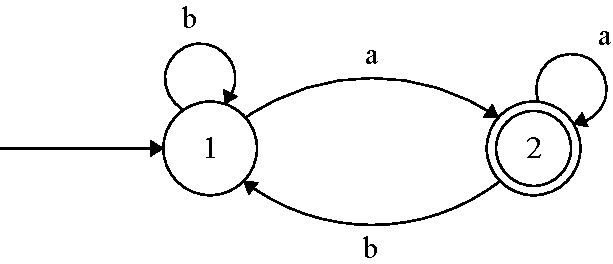
\includegraphics[width=0.6\textwidth]{Figures/DFA_example.pdf}
	\caption{Příklad deterministického automatu příjamjící slova obsahující písmena z abecedy \{a, b\} končící písmenem a}
	\label{fig:DFAex}
\end{figure}

\begin{figure}[!h]
	\centering
	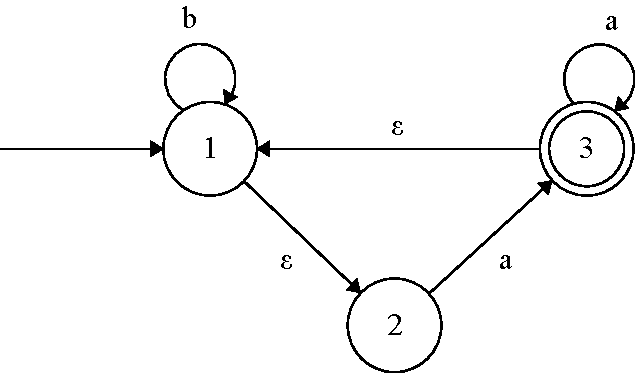
\includegraphics[width=0.6\textwidth]{Figures/NFA_example.pdf}
	\caption{Příklad nedeterministického automatu ekvivalentního k předchozímu deterministickému}
	\label{fig:NFAex}
\end{figure}

\section{Původ a vznik}
Regulární výrazy byly poprvé nadefinovány Americkým matematikem \textbf{Stephan Cole Kleene}, jako regulární jazyky. 
Dále se aplikovali v teoretické informatice, jako podkategorie \textbf{teorie automatů} a součást \textbf{formálních jazyků}.
Ačkoliv byli nadefinovány začátkem padesátých let, tak jejich využití v počítačích nastalo až na konci šedesátých let a to v 
jedním z nejznámějších operačních systémů UNIX.

\textbf{Ken Thompson} byl tím kdo navrhnul první implementaci využívanou v počítačích, která se používá do dnes. 
Tento algoritmus se pojmenoval \textbf{Thompson's construction} (Thompsonovo sestavení), který převádí textovou reprezentaci výrazu na ekvivalentní nedeterministický automat.